\documentclass[11pt]{article} % use larger type; default would be 10pt

\usepackage[utf8]{inputenc} % set input encoding (not needed with XeLaTeX)


\usepackage{geometry} % to change the page dimensions
\geometry{a4paper} % or letterpaper (US) or a5paper or....

\usepackage{graphicx} % support the \includegraphics command and options
\usepackage{amsmath}


\usepackage{booktabs} % for much better looking tables
\usepackage{array} % for better arrays (eg matrices) in maths
\usepackage{paralist} % very flexible & customisable lists (eg. enumerate/itemize, etc.)
\usepackage{verbatim} % adds environment for commenting out blocks of text & for better verbatim
\usepackage{subfig} % make it possible to include more than one captioned figure/table in a single float

\usepackage{fancyhdr} % This should be set AFTER setting up the page geometry
\pagestyle{fancy} % options: empty , plain , fancy
\renewcommand{\headrulewidth}{0pt} % customise the layout...
\lhead{}\chead{}\rhead{}
\lfoot{}\cfoot{\thepage}\rfoot{}

\usepackage{sectsty}
\allsectionsfont{\sffamily\mdseries\upshape} % (See the fntguide.pdf for font help)

\usepackage[nottoc,notlof,notlot]{tocbibind} % Put the bibliography in the ToC
\usepackage[titles,subfigure]{tocloft} % Alter the style of the Table of Contents
\renewcommand{\cftsecfont}{\rmfamily\mdseries\upshape}
\renewcommand{\cftsecpagefont}{\rmfamily\mdseries\upshape} % No bold!
\newcommand{\strong}[1]{\textbf{#1}}
\newcommand{\code}[1]{\texttt{#1}}
\newcommand{\st}{$^{\text{st}\ }$}
\newcommand{\nd}{$^{\text{nd}\ }$}
\newcommand{\rd}{$^{\text{rd}\ }$}
\newcommand{\nth}{$^{\text{th}\ }$}

\title{Assignment 6}
\author{Nathan Jervis - 1211159}

\begin{document}
\maketitle

\section{Question 6.1}

\subsection{Part A}

The miss rate is $\textbf{dataInBlock} = \frac{\textbf{dataSize}}{\textbf{blockSize}} = \frac{8}{64} = \frac{1}{8}$ or 12.5\%. The first address requested (0) is a miss, then that causes the next 64 bytes to be loaded (0-64). Then once an address outside of that block is needed Once the cache gets full (at adress 256KB)

All the misses are compulsory misses, since no address is ever requested twice, every address requested is a cold start cache miss.

\subsection{Part B}

The new miss rate is $\textbf{dataInBlock} = \frac{\textbf{dataSize}}{\textbf{blockSize}} = \frac{8}{32} = \frac{1}{4}$ or 25\%.

\subsection{Part C}

The new miss rate is $\textbf{dataInBlock} = \frac{\textbf{dataSize}}{\textbf{blockSize}} = \frac{8}{128} = \frac{1}{4}$ or 6.25\%.

\subsection{Part D}

With prefetching we'll only have the first cache miss, since we process blocks at the same rate we load them, the new block will always be ready by the time we need it. The only time it's not ready is when we first start. This means the cache miss rate is $\frac{\textbf{numberOfMisses}}{\textbf{numberOfMemoryAccess}} = \frac{\textbf{numberOfMisses}}{\frac{\textbf{TotalMemory}}{\textbf{MemoryAccessSize}}} = \frac{1}{\frac{2^{24}}{2^{3}}} = \frac{1}{2^{21}}$ or approximately 0\%.

This is a good thing. Do this.

\section{Question 6.2}

\subsection{Part A}

\begin{tabular}{|c|c|c|c|c|c|}\hline
Block Size: & 16 & 32 & 64 & 128 & 256\\\hline
Miss Rate & 8\% & 6\% & 4\% & 3.5\% & 3.2\%\\\hline
Miss Penalty & $30+10\cdot 16$ & $30+10\cdot 32$ & $30+10\cdot 64$ & $30+10\cdot 128$ & $30+10\cdot 256$ \\
& 190 & 350 & 670 & 1310 & 2590 \\\hline
Average Miss Penalty & 15.2 & 21 & 26.8 & 45.85 & 82.88\\\hline
\end{tabular}

The best block size for this penalty is 16

\subsection{Part B}

\begin{tabular}{|c|c|c|c|c|c|}\hline
Block Size: & 16 & 32 & 64 & 128 & 256\\\hline
Miss Rate & 8\% & 6\% & 4\% & 3.5\% & 3.2\%\\\hline
Miss Penalty & $36 + 16$ & $36+ 32$ & $36+ 64$ & $36+128$ & $36+ 256$ \\
& 52 & 68 & 100 & 164 & 292 \\\hline
Average Miss Penalty & 4.16 & 4.08 & 4 & 5.74 & 9.344 \\\hline
\end{tabular}

The best block size for this penalty is 64

\subsection{Part C}

\begin{tabular}{|c|c|c|c|c|c|}\hline
Block Size: & 16 & 32 & 64 & 128 & 256\\\hline
Miss Rate & 8\% & 6\% & 4\% & 3.5\% & 3.2\%\\\hline
Miss Penalty & 80 & 80 & 80 & 80 & 80 \\\hline
Average Miss Penalty & 6.4 & 4.8 & 3.2 & 2.8 & 2.56 \\\hline
\end{tabular}

The best block size for this penalty is 256

\section{Question 6.3}


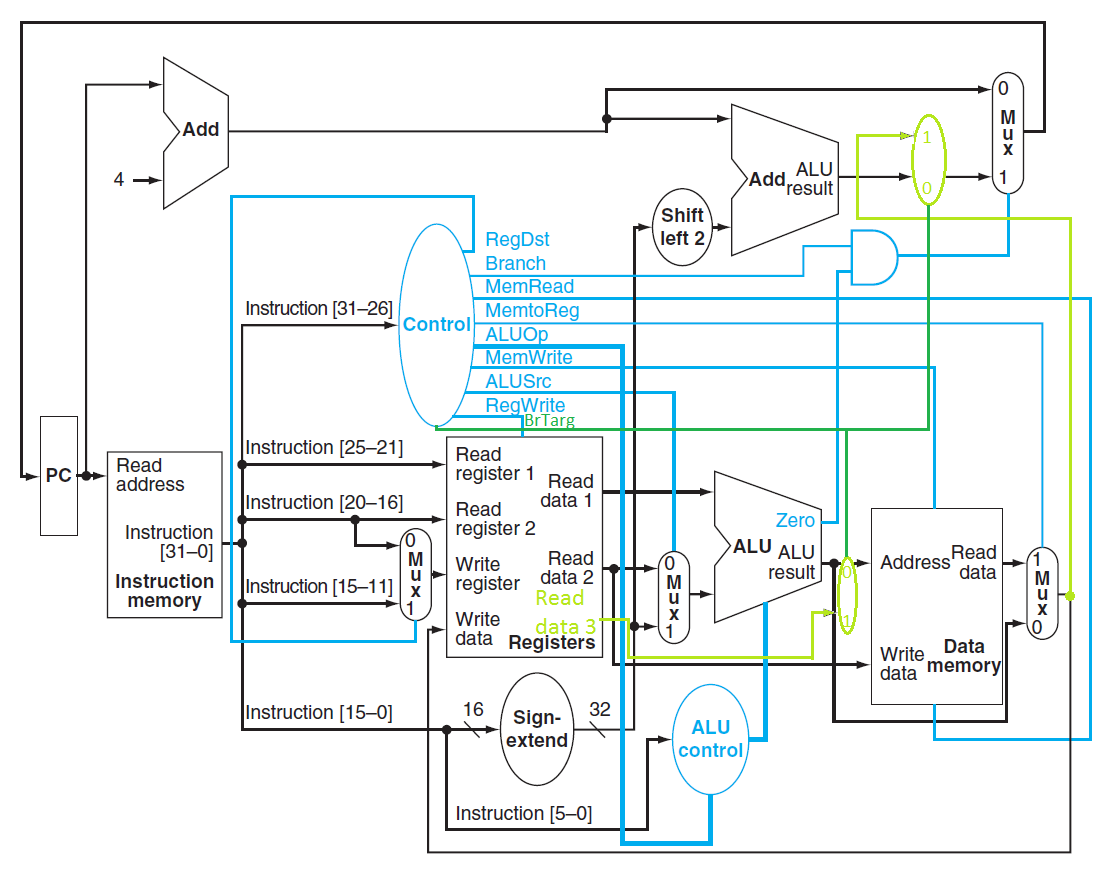
\includegraphics[width=\textwidth]{CPU.png}

We add a multiplexer to choose this 3\rd read register to read as the address. The 3\rd read register is selected by simply re-using the Write Register that is selected. Then the result of the memory load is moved to select between that and the immediate address. This is then selected between this and the regular program counter, based on the branch control bit and the zero of the ALU anded together.

\section{Question 6.4}

Submitted via avenue


\end{document}

